\chapter{Unidad 3. El núcleo y los procesos.}
El núcleo, conocido también como kernel, es el corazón del sistema operativo. Su función principal es gestionar de manera eficiente los recursos del sistema, como el procesador, la memoria, los dispositivos de entrada/salida (E/S), y otros recursos esenciales. El kernel actúa como intermediario entre el hardware y las aplicaciones que se ejecutan en el sistema, asegurando que los recursos se utilicen de manera óptima y que las aplicaciones puedan acceder a ellos de manera segura y controlada.

\begin{tcolorbox}
	\section{
		Funciones del Kernel}
	
	El kernel realiza varias funciones críticas en un sistema operativo:
	
	\textbf{Gestión del Procesador: }Coordina la asignación del tiempo de CPU a los diferentes procesos que se ejecutan en el sistema. Esto incluye la planificación de procesos y la conmutación de contexto entre procesos.
	
	\textbf{Gestión de la Memoria:} Supervisa y controla el acceso a la memoria principal. Esto incluye la asignación de memoria a los procesos, el manejo de la memoria virtual y la protección de la memoria para evitar que un proceso interfiera con otro.
	
	\textbf{
		Gestión de Entrada/Salida (E/S):} Controla las operaciones de entrada y salida, gestionando el acceso a dispositivos como discos duros, impresoras y otros periféricos. El kernel facilita la comunicación entre los dispositivos y los procesos que necesitan interactuar con ellos.
	
	\textbf{Gestión de Recursos: }Además de CPU, memoria y dispositivos de E/S, el kernel también administra otros recursos del sistema, como el sistema de archivos, la seguridad y la gestión de usuarios.


\end{tcolorbox}
\section{Procesos}

Uno de los conceptos más fundamentales en la gestión de un sistema operativo es el de \textbf{proceso}. El concepto de proceso se originó con la llegada de la \textit{multiprogramación}, que permitió la ejecución simultánea de múltiples programas en un mismo sistema. Esta capacidad transformó la forma en que los sistemas operativos gestionan los recursos y las tareas que se llevan a cabo en un ordenador.

Consideremos el caso de una computadora portátil moderna. Desde el momento en que se enciende, el sistema operativo comienza a ejecutar una serie de procesos en segundo plano, muchos de los cuales el usuario ni siquiera nota. Por ejemplo, se inician procesos como el explorador de Windows, servicios esenciales como los de red e impresión, procesos de seguridad como el antimalware, servidores de bases de datos, y la Máquina Virtual de Java (JVM) si el entorno está configurado para desarrollo con Java. Mientras estos procesos se ejecutan, el usuario puede estar navegando por internet o escuchando música, sin darse cuenta de la complejidad de las operaciones que ocurren simultáneamente.
\begin{figure}[H]
	\centering
	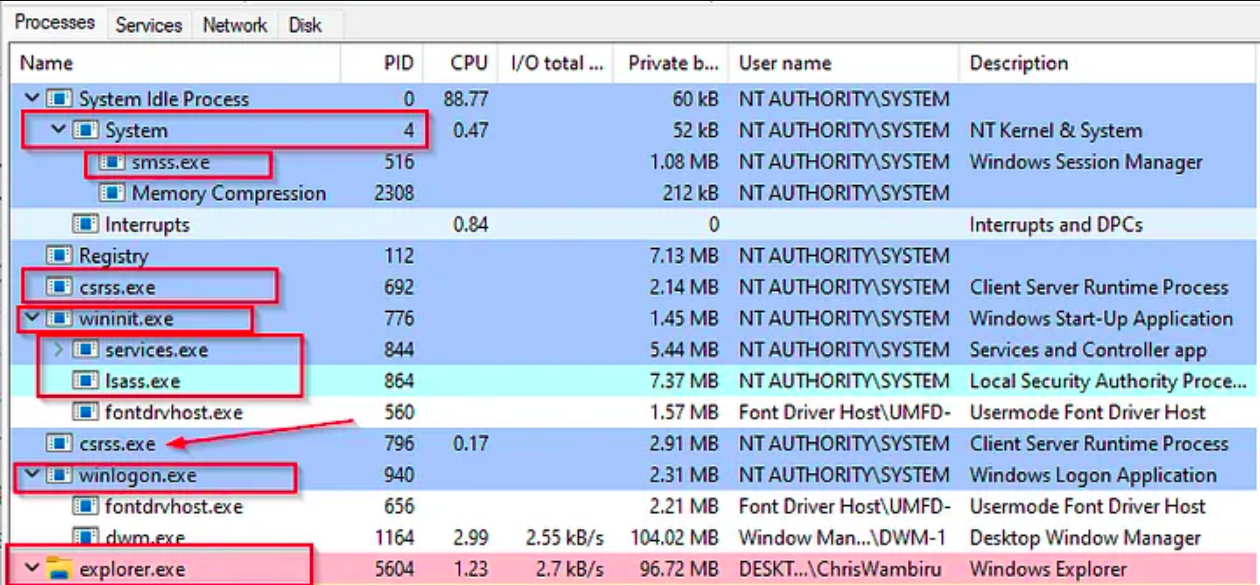
\includegraphics[width=0.8\linewidth]{Imagenes/procesos.png}
	\caption{Procesos que se inician al arrancar windows. }
	\label{fig:enter-label}
\end{figure}

Toda esta actividad debe ser gestionada de manera eficiente, y es aquí donde entra en juego la multiprogramación con soporte para múltiples procesos. Esta técnica permite que el sistema operativo administre los recursos del procesador, la memoria y otros dispositivos, de manera que varios procesos puedan ejecutarse ``al mismo tiempo'' sin interferir unos con otros.

Podemos, entonces, definir a un \textbf{proceso} como:

\begin{tcolorbox}
	\textbf{Una instancia de un programa en ejecución.}
\end{tcolorbox}

Un proceso no es solo un programa almacenado en disco o en la memoria, sino una entidad activa que está utilizando los recursos del sistema para llevar a cabo tareas específicas. Cada proceso tiene su propio espacio de memoria, su estado, y es gestionado por el sistema operativo para asegurar que todos los procesos puedan operar de manera eficiente y segura dentro del sistema.
\begin{table}[H]
	\centering
	\rowcolors{2}{gray!25}{white}
	\begin{tabularx}{0.9\textwidth}{|X|X|}
		\hline
		\textbf{Programa} & \textbf{Proceso} \\ \hline
		Conjunto de instrucciones almacenadas en disco o memoria. & Instancia de un programa en ejecución. \\ \hline
		Es un archivo pasivo, sin interacción con el hardware hasta que se ejecuta. & Es una entidad activa que utiliza recursos del sistema como CPU, memoria, etc. \\ \hline
		No tiene estado hasta que se inicia su ejecución. & Tiene un estado (listo, en ejecución, en espera, etc.) que cambia dinámicamente. \\ \hline
		Es estático, no cambia una vez escrito. & Es dinámico, ya que las instrucciones se están ejecutando y puede cambiar con el tiempo. \\ \hline
		Puede existir en disco duro o en memoria como código fuente o compilado. & Existe en la memoria principal y se asocia a un identificador único (PID). \\ \hline
		No consume recursos del sistema operativo por sí mismo. & Consume recursos como tiempo de CPU, espacio en memoria, y otros mientras se ejecuta. \\ \hline
	\end{tabularx}
	\caption{Diferencias entre un programa y un proceso}
	\label{tabla_programa_proceso}
\end{table}
\subsection{El modelo del proceso}

El modelo del proceso describe cómo el sistema operativo maneja la ejecución de programas. Este modelo es fundamental para entender cómo los programas se convierten en procesos activos en el sistema y cómo se gestionan durante su ciclo de vida.

En el modelo de procesos, cada proceso se concibe como una entidad que contiene:

\begin{itemize}
	\item \textbf{Código del programa}: Las instrucciones que el proceso ejecutará.
	\item \textbf{Datos}: Las variables necesarias para la ejecución.
	\item \textbf{Recursos del sistema}: CPU, memoria, dispositivos de E/S, que el proceso necesita para funcionar.
\end{itemize}

Para entender mejor el \textbf{modelo del proceso}, podemos utilizar la siguiente analogía de un taller mecánico:

\subsubsection{Analogía: Taller Mecánico}
\begin{tcolorbox}
	\begin{enumerate}
		\item \textbf{Vehículo en el Taller (Proceso):} Imagina que cada proceso es un vehículo que llega a un taller mecánico para ser reparado o mantenido. Este vehículo representa una instancia de un programa que ha sido \textit{activado} y ahora requiere atención.
		
		\item \textbf{Mecánico (Procesador):} El mecánico del taller es como el procesador del sistema, encargado de realizar las reparaciones necesarias. Este mecánico debe seguir un conjunto de instrucciones específicas (el programa) para reparar el vehículo.
		
		\item \textbf{Manual de Reparaciones (Programa):} El mecánico consulta un manual de reparaciones, que contiene todas las instrucciones necesarias para realizar la reparación. Este manual es análogo al código del programa que el proceso necesita ejecutar.
		
		\item \textbf{Herramientas y Piezas (Recursos del Sistema):} Para llevar a cabo las reparaciones, el mecánico necesita herramientas y piezas de recambio, que en el sistema operativo corresponden a los recursos del sistema, como la CPU, memoria, y dispositivos de entrada/salida.
		
		\item \textbf{Ejecución del Proceso:} Mientras el vehículo está en el taller, el mecánico trabaja en él, siguiendo el manual, utilizando las herramientas y asegurándose de que la reparación se realice correctamente. Esto es similar a cómo un proceso se ejecuta en un sistema operativo, siguiendo las instrucciones del programa y utilizando los recursos disponibles.
	\end{enumerate}
\end{tcolorbox}

La idea clave es que un proceso es una actividad de cierto tipo: tiene un programa, una entrada, una salida y un estado. Varios procesos pueden compartir un solo procesador mediante el uso de un algoritmo de planificación para determinar cuándo se debe detener el trabajo en un proceso para dar servicio a otro.


\subsection{Bloque de control de procesos (PCB)}

Desde el punto de vista del sistema operativo, un proceso se representa como un conjunto de datos que describe su estado en cada momento, los recursos utilizados, los registros, y otra información relevante. Este conjunto de datos se denomina \textbf{Bloque de control de procesos} (\textbf{PCB}, por sus siglas en inglés: \textit{Process Control Block}).

El PCB es fundamental para la gestión de procesos en un sistema operativo, ya que contiene toda la información necesaria para controlar y administrar un proceso. Cada proceso en el sistema tiene su propio PCB, y estos se almacenan en una estructura de datos que el sistema operativo utiliza para llevar un seguimiento preciso de todos los procesos.

A continuación, se detallan los componentes clave que suelen incluirse en un PCB:

\begin{tcolorbox}
	\begin{itemize}
		\item \textbf{Identificador del proceso (PID):} Un número único que identifica a cada proceso en el sistema.
		\item \textbf{Estado del proceso:} El estado actual del proceso, que puede ser en ejecución, preparado, bloqueado, suspendido bloqueado y suspendido preparado; el estado del proceso también contiene información relativa a la prioridad del proceso.
		\item \textbf{Contador de programa \textit{(Program Counter)} (PC):} La dirección de la siguiente instrucción que se ejecutará para este proceso.
		\item \textbf{Registros de la CPU:} Incluye el contenido de los registros del procesador utilizados por el proceso, como los registros generales, punteros de pila, registros de estado, entre otros.
		\item \textbf{Información de gestión de memoria:} Detalles sobre la memoria asignada al proceso, incluyendo las tablas de páginas o segmentos.
		\item \textbf{Información de gestión de recursos:} Información sobre los recursos que el proceso está utilizando, como archivos abiertos, dispositivos de E/S, y otras asignaciones de recursos.
		\item \textbf{Información de contabilidad del proceso:} Datos sobre el uso de la CPU, límites de tiempo, y otra información relevante para la contabilidad del sistema.
	\end{itemize}
\end{tcolorbox}

Estas informaciones se encuentran en memoria o disco, y se accede a ellas en los momentos en que se hace necesaria su actualización o consulta.

El PCB es esencial para la conmutación de contexto, que es el proceso mediante el cual el sistema operativo guarda el estado de un proceso y carga el estado de otro.

\subsubsection{Cambio de proceso: conmutación de contexto}

Cuando un sistema operativo decide que un proceso debe dejar de ejecutarse y otro debe comenzar, realiza lo que se llama una \textbf{conmutación de contexto}. Este proceso implica los siguientes pasos:

\begin{tcolorbox}


\begin{enumerate}
	\item \textbf{Guardar el Estado del Proceso Actual:} El sistema operativo utiliza el PCB para almacenar el estado completo del proceso actual. Esto incluye el contador de programa, los registros de la CPU, y cualquier otra información relevante. Esta acción asegura que el proceso pueda reanudarse más tarde exactamente desde donde fue interrumpido.
	
	\item \textbf{Cargar el Estado del Nuevo Proceso:} Una vez que se ha guardado el estado del proceso actual, el sistema operativo selecciona el siguiente proceso que debe ejecutarse. Utilizando el PCB de este nuevo proceso, el sistema operativo carga el estado que había sido almacenado anteriormente.
	
	\item \textbf{Actualizar el Contador de Programa y Registros:} El contador de programa y los registros de la CPU se actualizan con la información del nuevo proceso. Esto le permite al procesador continuar la ejecución del nuevo proceso desde el punto donde fue pausado o desde su inicio.
	
	\item \textbf{Reanudar la Ejecución:} Con el estado del nuevo proceso cargado, el sistema operativo cede el control del CPU a este proceso, permitiéndole reanudar o iniciar su ejecución.
\end{enumerate}

\end{tcolorbox}

Este proceso de conmutación de contexto es rápido y eficiente, pero también implica una cierta sobrecarga, ya que el sistema operativo debe realizar varias operaciones para asegurar que los procesos se gestionen de manera correcta y continua.

En resumen, la conmutación de contexto y el PCB permiten al sistema operativo manejar múltiples procesos de manera ordenada, asegurando que cada proceso pueda avanzar en su ejecución sin interferir con los demás.




\subsection{Estado de los procesos}

En un sistema operativo, cada proceso pasa por una serie de estados durante su ciclo de vida. Estos estados determinan la condición del proceso en un momento dado y cómo el sistema operativo debe gestionarlo. Los \textbf{Bloques de Control de Procesos (PCB)} se almacenan en colas, cada una de las cuales representa un estado particular del proceso. Es importante destacar que los estados de los procesos son internos al sistema operativo y, por lo tanto, transparentes para el usuario.

\begin{figure}[H]
	\centering
	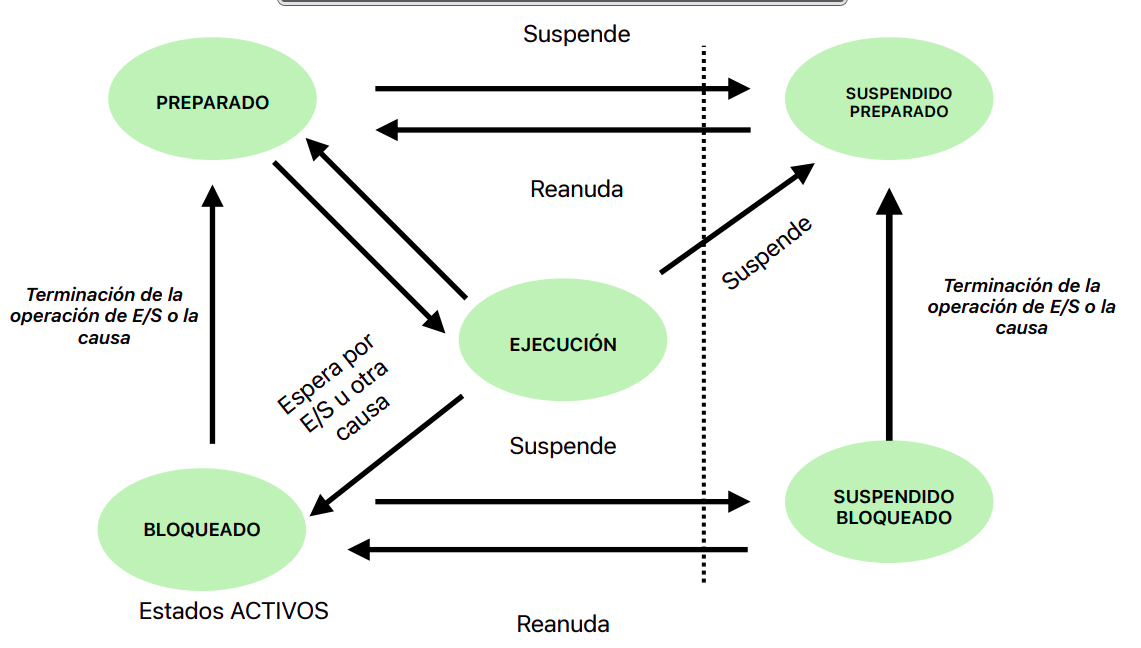
\includegraphics[width=0.8\linewidth]{Imagenes/procesosesquema.png}
	\caption{Estado de los procesos y sus transiciones. }
	\label{fig:enter-label}
\end{figure}

Los estados de los procesos se pueden dividir en dos categorías principales: \textbf{activos} e \textbf{inactivos}.

\newpage
\subsubsection{Estados activos}

Los estados activos son aquellos en los que un proceso está involucrado directamente en la ejecución o está preparado para ejecutarse. Estos estados incluyen:

\begin{tcolorbox}
\begin{itemize}
	\item \textbf{En ejecución:} El proceso está actualmente utilizando la CPU para ejecutar sus instrucciones. En este estado, el procesador está ocupado realizando las tareas definidas por el proceso. 
	
	\textbf{Ejemplo:} Si estás utilizando un editor de texto para escribir un documento, el proceso que maneja el editor de texto está en ejecución cuando estás escribiendo activamente.
	
	\item \textbf{Preparado:} El proceso está listo para ejecutarse y está esperando que el sistema operativo le asigne la CPU. Los procesos en este estado se encuentran en la cola de procesos listos. 
	
	\textbf{Ejemplo:} Si tienes varias pestañas abiertas en un navegador, los procesos que manejan las pestañas inactivas están en el estado de preparado, esperando su turno para recibir tiempo de CPU.
	
	\item \textbf{Bloqueado:} El proceso no puede continuar su ejecución hasta que se cumpla una condición externa, como la finalización de una operación de entrada/salida (E/S) o la disponibilidad de un recurso. A pesar de estar en espera, el proceso sigue siendo considerado ``activo'' porque se espera que retome la ejecución tan pronto como la condición que lo bloquea se resuelva.
	
\end{itemize}
\end{tcolorbox}

\subsubsection{Estados inactivos}

Los estados inactivos son aquellos en los que un proceso no está utilizando la CPU y ha sido suspendido temporalmente por el sistema operativo. Estos estados incluyen:

\begin{tcolorbox}
\begin{itemize}
	\item \textbf{Suspendido bloqueado:} El proceso estaba en el estado de \textit{Bloqueado} pero ha sido movido a la memoria secundaria (swap) debido a que el sistema necesita liberar espacio en la memoria principal. En este estado, el proceso no puede avanzar ni siquiera cuando se resuelve la condición que lo bloqueaba, hasta que sea devuelto a la memoria principal.
	
	
	\item \textbf{Suspendido preparado:} El proceso estaba en el estado de \textit{Preparado} y ha sido movido a la memoria secundaria. A diferencia del estado \textit{Suspendido Bloqueado}, este proceso está listo para ejecutarse tan pronto como sea devuelto a la memoria principal y reciba tiempo de CPU.

\end{itemize}

\end{tcolorbox}

La clasificación de los estados de los procesos en activos e inactivos permite al sistema operativo gestionar de manera eficiente los recursos y la ejecución de los procesos. Los estados activos indican que el proceso está participando activamente en la ejecución o está preparado para hacerlo, mientras que los estados inactivos indican que el proceso ha sido suspendido temporalmente y no está en memoria principal.

\newpage
\subsection{Transiciones de estado}
Todo proceso a lo largo de su vida puede cambiar de estado varias veces. cada uno de estos cambios se llama \textbf{transición de estado}. Estas transiciones son las siguientes:
\begin{tcolorbox}
	
	
	\begin{itemize}
		\item \subsubsection {Comienzo de la ejecución}
		Todo proceso comienza cuando se emite la orden de ejecución del programa. Inicialmente, el proceso se inserta en la \textbf{cola de preparados}. El encolamiento de procesos en esta cola dependerá de la política de gestión que utilice el sistema operativo.
		
		\item \subsubsection {Paso a estado de ejecución}
		Cuando el procesador se encuentra inactivo y en la cola de preparados existe algún proceso en espera de ser ejecutado, el primer proceso en la cola es seleccionado y se le asigna la CPU, cambiando su estado a \textbf{en ejecución}.
		
			\item \subsubsection {Paso a estado bloqueado}
		Un proceso en ejecución puede necesitar realizar una operación de entrada/salida (E/S), como leer un archivo desde el disco. En este caso, debido a que la operación de E/S puede tardar en completarse, el proceso no puede continuar ejecutándose inmediatamente. Por lo tanto, se cambia su estado a \textbf{bloqueado} y su PCB se inserta en la \textbf{cola de bloqueados}.
		
				\item \subsubsection{Paso a estado preparado}
		Un proceso puede pasar al estado preparado desde varios otros estados, bajo las siguientes circunstancias:
		
		\begin{itemize}
			\item \textbf{Orden de ejecución de un programa:} Cuando se inicia un nuevo proceso, se inserta en la cola de preparados.
			\item \textbf{Finalización de una operación de E/S:} Si un proceso estaba bloqueado esperando la finalización de una operación de E/S, una vez que la operación se completa, el proceso se mueve de la \textbf{cola de bloqueados} a la \textbf{cola de preparados}.
			\item \textbf{Interrupción del proceso en ejecución:} Si un proceso en ejecución es interrumpido (por ejemplo, por una interrupción de hardware o por el sistema operativo), su estado cambia a preparado, y su PCB se mueve a la \textbf{cola de preparados}.
			\item \textbf{Activación de un proceso suspendido:} Un proceso previamente suspendido (sin estar bloqueado) puede ser reactivado, lo que lo moverá a la cola de preparados.
		\end{itemize}
		

						\end{itemize}	
	\end{tcolorbox}	






\begin{tcolorbox}


	\begin{itemize}
		
		
	
		
	
		

	

	
		
		\item \subsubsection {Paso a estado suspendido bloqueado}
		Si un proceso está bloqueado y el sistema operativo necesita liberar memoria o suspender el proceso por alguna razón, el proceso es movido a estado \textbf{suspendido bloqueado}. Su PCB se traslada a la \textbf{cola de procesos suspendidos bloqueados}.
		
		\begin{itemize}
			\item \textbf{Ejemplo:} Un proceso que estaba esperando la respuesta de una operación de red puede ser suspendido si el sistema operativo necesita liberar recursos. 
		\end{itemize}
		
			\item \subsubsection{Paso a estado suspendido preparado} 
		Un proceso puede pasar a este estado en tres circunstancias diferentes:
		
		\begin{itemize}
			\item \textbf{Suspensión de un proceso preparado:} Un proceso en la cola de preparados puede ser suspendido, moviéndose así a la \textbf{cola de suspendidos preparados}.
			\item \textbf{Suspensión de un proceso en ejecución:} Si un proceso en ejecución es suspendido, su estado cambia a suspendido preparado, y su PCB se mueve a la cola de suspendidos preparados.
			\item \textbf{Desbloqueo de un proceso suspendido bloqueado:} Si se elimina la causa que bloqueaba un proceso suspendido bloqueado, este proceso se moverá a la cola de suspendidos preparados.
		\end{itemize}
		
	\end{itemize}
\end{tcolorbox}





\subsection{Operaciones sobre procesos}

Los sistemas operativos modernos proporcionan varias funciones para manipular y gestionar los procesos. A continuación, se describen las principales operaciones que se pueden realizar sobre un proceso:


\begin{tcolorbox}

\begin{itemize}
	\item \textbf{Crear un proceso:}
	La creación de un proceso se inicia mediante la orden de ejecución de un programa. Este proceso requiere varios argumentos, como el nombre del proceso y su prioridad. En este momento, se crea el \textbf{Bloque de Control de Procesos (PCB)}, que se inserta en la \textbf{cola de procesos preparados}.
	
	\begin{itemize}
		\item \textbf{Creación jerárquica:} En este tipo de creación, cada proceso que se crea es hijo del proceso creador y hereda el entorno de ejecución de su padre. Por ejemplo, el primer proceso que ejecuta un usuario suele ser hijo del intérprete de comandos con el que interactúa.
		\item \textbf{Creación No Jerárquica:} En esta modalidad, cada proceso creado por otro proceso se ejecuta independientemente de su creador y con un entorno diferente. Este tipo de creación no es común en los sistemas operativos modernos.
	\end{itemize}
	
	\item \textbf{Destruir un proceso:}
	La destrucción de un proceso implica la eliminación del proceso mediante una orden específica. Esta operación resulta en la eliminación del PCB asociado con el proceso.
	

	
	\end{itemize}
	
	\end{tcolorbox}
	
	
	\begin{itemize}
		
	\begin{tcolorbox}


	
	\item \textbf{Suspender un proceso:}
	La suspensión de un proceso es una operación de alta prioridad que paraliza el proceso, permitiendo que pueda ser reanudado posteriormente. Esta operación es útil en situaciones de malfuncionamiento o sobrecarga del sistema.
	

	
	\item \textbf{Reanudar un proceso:}
	La reanudación de un proceso se refiere a la activación de un proceso que ha sido previamente suspendido, permitiendo que continúe su ejecución desde el punto en el que fue interrumpido.
	

	
	\item \textbf{Cambiar la prioridad de un proceso:}
	Esta operación permite ajustar la prioridad de un proceso en ejecución, lo que puede afectar el orden en el que el proceso recibe tiempo de CPU en comparación con otros procesos.
	

	
	\item \textbf{Temporizar la ejecución de un proceso:}
	La temporización de un proceso controla su ejecución en función de un periodo de tiempo fijo, permitiendo que el proceso se ejecute en intervalos regulares o en una sola vez después de un período determinado.
	

	
	\item \textbf{Despertar un proceso:}
	Despertar un proceso se refiere a desbloquear un proceso que ha sido previamente bloqueado debido a la temporización u otras causas.
	

	
		\end{tcolorbox}
	
\end{itemize}



\subsection{Prioridades}


En un sistema operativo, cada proceso tiene asignada una prioridad que determina cómo y con qué frecuencia puede acceder al procesador en comparación con otros procesos. Esta prioridad refleja las necesidades de ejecución del proceso en cuanto a urgencia y asignación de recursos, influenciando directamente el orden y la velocidad con la que se ejecutan los procesos en el sistema.

Las prioridades se pueden clasificar de diferentes maneras, según cómo se asignan y si pueden o no modificarse durante la ejecución del proceso.




\begin{itemize}
	\item \textbf{Clasificación según la asignación de la prioridad:}
	\begin{itemize}
		\begin{tcolorbox}

	
		\item \textbf{Asignadas por el sistema operativo:}
		Estas prioridades son asignadas automáticamente por el sistema operativo en el momento en que el proceso comienza su ejecución. La asignación de estas prioridades depende principalmente de los privilegios del propietario del proceso y del modo de ejecución en el que se encuentra.
		
		\begin{itemize}
			\item \textbf{Ejemplo:} Un proceso iniciado por un administrador del sistema puede recibir una prioridad más alta que un proceso iniciado por un usuario regular.
		\end{itemize}
		
		\item \textbf{Asignadas por el propietario:}
		En este caso, es el propio usuario quien asigna la prioridad con la que un proceso debe ejecutarse. Este enfoque es común en sistemas de tiempo real, donde ciertos procesos necesitan responder rápidamente a eventos sin ser interrumpidos.
		
		\begin{itemize}
			\item \textbf{Ejemplo:} En un sistema de control industrial, un usuario podría asignar una alta prioridad a un proceso que monitorea la temperatura, asegurando que no se demore su ejecución.
		\end{itemize}
			\end{tcolorbox}
	\end{itemize}
	
	\newpage
	\item \textbf{Clasificación según la variabilidad de la prioridad:}
	\begin{itemize}
		\begin{tcolorbox}

		\item \textbf{Estáticas:}
		Las prioridades estáticas son aquellas que no pueden ser modificadas durante la ejecución del proceso. Una vez que se asigna una prioridad estática, permanece constante durante todo el ciclo de vida del proceso. Este tipo de prioridad es utilizado en sistemas de tiempo compartido, donde la equidad en la asignación de recursos es importante, pero no en sistemas de tiempo real, donde la flexibilidad y la capacidad de respuesta rápida son cruciales.
		
		\begin{itemize}
			\item \textbf{Ejemplo:} Un proceso de mantenimiento del sistema que tiene una prioridad estática podría estar programado para ejecutarse con regularidad, sin cambios en su prioridad.
		\end{itemize}
		
		\item \textbf{Dinámicas:}
		Las prioridades dinámicas pueden ser modificadas durante la ejecución del proceso. Este ajuste permite que el sistema operativo reaccione a eventos cambiantes, ajustando la prioridad de los procesos para asegurar que se manejen adecuadamente.
		
		\begin{itemize}
			\item \textbf{Ejemplo:} Si un proceso de baja prioridad requiere atención urgente debido a un evento crítico, el sistema operativo puede elevar temporalmente su prioridad para asegurar que se maneje rápidamente.
		\end{itemize}
		
		\end{tcolorbox}
	\end{itemize}
\end{itemize}

\subsection{Tipos de procesos}

Los procesos en un sistema operativo se pueden clasificar en varias categorías según diferentes criterios, como el uso que se les dará, cómo se construyó el código ejecutable, su capacidad de acceso a los recursos, y su forma de ejecución. A continuación, se describen los principales tipos de procesos:

\begin{itemize}
	
	
	
	\item \textbf{Clasificación según el uso y la construcción del código ejecutable:}
	
	

	
	\begin{itemize}
		\begin{tcolorbox}
		\item \textbf{Reutilizables:}
		Estos procesos pueden cambiar los datos que utilizan, pero si se vuelven a ejecutar, necesitan comenzar en su estado inicial y procesar nuevos datos. Este tipo de procesos es común en los programas normales del usuario.
		
		\begin{itemize} 
			\item \textbf{Ejemplo: }Un videojuego, donde un usuario nuevo genera una nueva partida.
		\end{itemize}
		
		\item \textbf{Reentrantes:}
	Los procesos reentrantes son programas que pueden ser utilizados por varios usuarios o tareas al mismo tiempo sin que se interfieran entre ellos. Esto es posible porque no guardan datos que cambien en su memoria; en lugar de eso, cada usuario o tarea tiene su propio espacio para manejar sus datos, mientras todos comparten el mismo código del programa.
		
		\begin{itemize}
			\item \textbf{Ejemplo:} Una calculadora online, permite muchos usuarios de manera "simultánea".
		\end{itemize}
	\end{tcolorbox}
	\end{itemize}
	
	\newpage
	\item \textbf{Clasificación según la capacidad de acceso a los recursos:}
	
	\begin{itemize}
		\begin{tcolorbox}
		\item \textbf{Apropiativos:}
		Los procesos apropiativos son aquellos que, una vez que tienen asignado un recurso, no permiten que otro proceso acceda a ese recurso hasta que hayan terminado de utilizarlo.
		
		\begin{itemize}
			\item \textbf{Ejemplo:} Una impresora; mientras el proceso utiliza la impresora, no permite que otro proceso pueda acceder a ella.
		\end{itemize}
		
		\item \textbf{No Apropiativos:}
		Los procesos no apropiativos permiten que otros procesos accedan a un recurso que están utilizando, lo que facilita el uso compartido de recursos entre múltiples procesos.
		
		\begin{itemize}
			\item \textbf{Ejemplo:} Un proceso que utiliza una base de datos en modo compartido es un proceso no apropiativo, ya que permite que otros procesos accedan a la misma base de datos simultáneamente.
		\end{itemize}
	\end{tcolorbox}
	\end{itemize}
	
	
	
	
	\item \textbf{Clasificación según la forma de ejecución:}
	
	\begin{itemize}
		
		\begin{tcolorbox}


		\item \textbf{Residentes:}
		Los procesos residentes son aquellos que permanecen en la memoria principal durante todo el tiempo que dure su ejecución.
		
	
		
		\item \textbf{Intercambiables:}
		Los procesos intercambiables pueden ser llevados desde la memoria principal al disco mientras están bloqueados. La memoria principal liberada por estos procesos puede ser utilizada por otros procesos que la necesiten en ese momento.
	
		
			\end{tcolorbox}
	\end{itemize}
	

	
\end{itemize}

\newpage

\subsection{Excepciones}

A lo largo de la ejecución de un proceso, pueden surgir una serie de irregularidades o fallos que el sistema operativo debe controlar y, si es posible, corregir. Estos problemas, conocidos como excepciones, pueden ser de diversa naturaleza y afectar al proceso de diferentes maneras. Entre los tipos de excepciones que pueden ocurrir, se incluyen:

\begin{itemize}
	\begin{tcolorbox}
		
	\item \textbf{Fallos de hardware:} Problemas físicos con los componentes del sistema, como fallos en la memoria o en los dispositivos de entrada/salida.
	\item \textbf{Fallos de software:} Errores en el código del programa que pueden interrumpir su correcta ejecución.
	\item \textbf{Entrada de datos incorrectos:} Datos proporcionados al programa que no cumplen con el formato o el tipo esperado.
	\item \textbf{Eventos anómalos:} Situaciones inesperadas que no se contemplaban en el diseño del programa, como la pérdida de conexión a un servidor.
	\end{tcolorbox}
\end{itemize}

Para gestionar estos eventos, los sistemas operativos incorporan lo que se denomina un \textbf{gestor de excepciones}. La misión del gestor de excepciones es controlar el software que maneja este tipo de eventos o excepciones, intentando corregirlos o, en su defecto, minimizando su impacto en el sistema.

Según la gravedad de los eventos que pueden presentarse, las excepciones se dividen en tres categorías principales:

\begin{itemize}
	\item \textbf{Errores catastróficos:} 
	Estos son errores que imposibilitan el funcionamiento del sistema operativo y no hay forma de recuperarlo. Un ejemplo de un error catastrófico sería un fallo en la tensión de alimentación del hardware, que podría provocar que el sistema se apague inesperadamente y no pueda reiniciarse correctamente.
	
	\item \textbf{Errores no recuperables:} 
	Estos errores, aunque no afectan al sistema operativo en su totalidad, impiden que el proceso afectado continúe con su ejecución. Un ejemplo típico es la aparición de una división por cero en un cálculo matemático, lo que provoca la interrupción inmediata del proceso.
	
	\item \textbf{Errores recuperables:} 
	Son errores que, con ciertos ajustes o correcciones, permiten que el proceso continúe su ejecución normal. Un ejemplo podría ser la introducción de datos en un formato incorrecto, que el sistema operativo puede corregir o solicitar nuevamente la información para evitar la interrupción del proceso.
\end{itemize}


